\section[MEX 2-3: Pressure driven percolation]{Model Exercise 2-3 (04): Effect of compressibility on pressure driven percolation}
\label{sec:mex04}
%------------------------------------------------------------------------------
\Authors{Mathias Nest, Amir Shoarian Sattari, Keita Yoshioka et al.}
%------------------------------------------------------------------------------
\subsection{Model set-up}
%------------------------------------------------------------------------------
Salt barriers do not only protect mines against the intrusion of ground water, but they can also be important to keep substances securely isolated in underground repositories and reservoirs. Examples include caverns for gas and oil, as well as repositories for toxic or radioactive waste. In this model exercise we look at the difference between the pressure driven percolation of liquids and gases, which is not only due to their different viscosities, but also to their different response to a change in the available volume. 

Liquids like brine react with a large change in pressure, because of their rather high bulk modulus $K$:
\begin{equation}
dp = -K \frac{dV}{V}
\end{equation}
Gases, which can be described approximately with the ideal gas equation
\begin{equation}
pV=nRT
\end{equation}
show a far smaller change in pressure. In this model exercise we explore this difference in a setup similar to the one in MEX 2, under the assumption, that there is only a finite amount of substance available to spread into the rock salt. Another way to put this is, that a lab-scale model of the in-situ experiment MEX 11 is set up. 

The basic reasoning behind the exercise is as follows: The total mass of the brine or gas is conserved, and consists of the mass in the reservoir $M_R$, the mass on the interfaces of the grains $M_I$, and the mass $M_L$ that has leaked out of the sample.
\begin{equation}
M = M_R + M_I + M_L \quad \mbox{= conserved}
\end{equation}
$M_I$ is part of the model, $M_L$ can be calculated using absorbing boundaries at the surface of the sample, at from the knowledge of the total amount $M$ that is present initially, the mass that remains in the reservoir $M_R$ can be calculated. This way, it is not necessary to model the reservoir (gas cylinder or brine container) explicitly. From the changing $M_R$ under the assumption of a fixed reservoir volume the change of the pressure in the reservoir, which drives the pressure driven percolation, can be calculated. Initially, at time $t=0$, $M_I=M_L=0$, and the pressure in the reservoir is high enough to open pathways between grains. Then, pressures and the extent of the distribution of the substances is monitored. 

\begin{figure}[!ht]
\centering
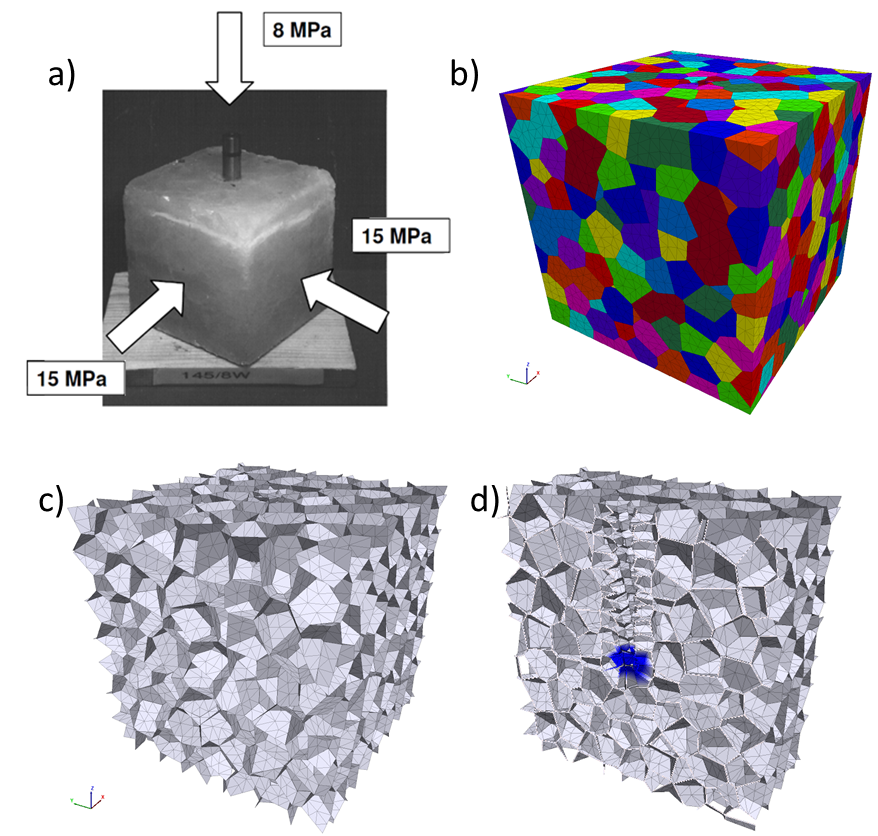
\includegraphics[width=1\textwidth]{figures/mex4-dem-setup.png}
\caption{a) Stress boundary condition b) discrete grain structure of 3DEC model c) grain boundaries/interfaces d) initial pressure on grain boundaries}
\label{fig:ME4-dem-setup}
\end{figure}

%------------------------------------------------------------------------------
\subsection{Model approaches}
%------------------------------------------------------------------------------
\subsubsection*{Discrete-Element-Method (DEM)}

For the numerical model in 3DEC the same setup was used as in MEX 2, see Fig. \ref{fig:ME4-dem-setup}. An initial reservoir pressure $p_R$ of 12 MPa, between principal stress $\sigma_2$ and $\sigma_3$, was chosen, to allow percolation. The bulk modulus of the brine was set to 2 GPa. Various reservoir volumes were tested, and  $V_R$ = 13 litres was found to give the clearest difference between gas and liquid.
For the simulation the masses $M_I$ and $M_L$ were calculated every 25 timesteps. From this, the mass in the reservoir was calculated, and converted into a pressure by the constitutive relations above. The new reservoir pressure was then applied as an updated boundary condition as shown in Fig. \ref{fig:ME4-dem-setup} d). 

\begin{figure}[!ht]
\centering
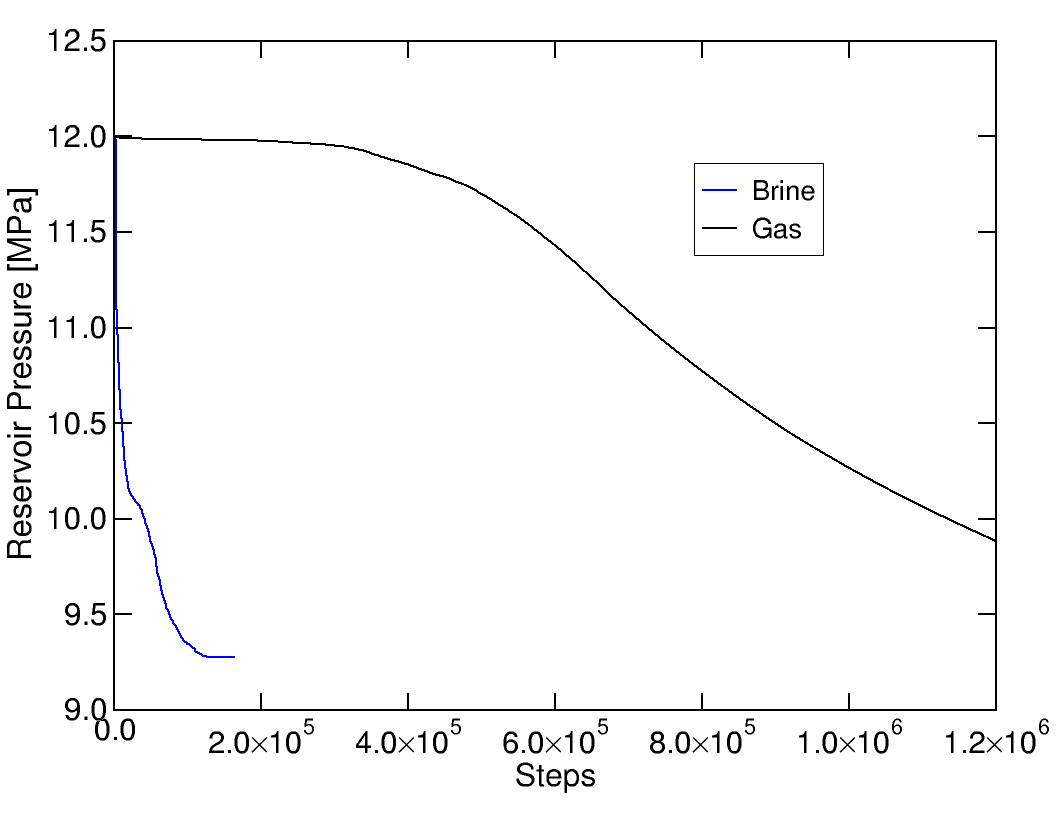
\includegraphics[width=1\textwidth]{figures/me4-3dec-comparison.png}
\caption{Pressure evolution in a finite size gas/liquid reservoir.}
\label{fig:ME4-3dec-comp}
\end{figure}

\begin{figure}[!ht]
\centering
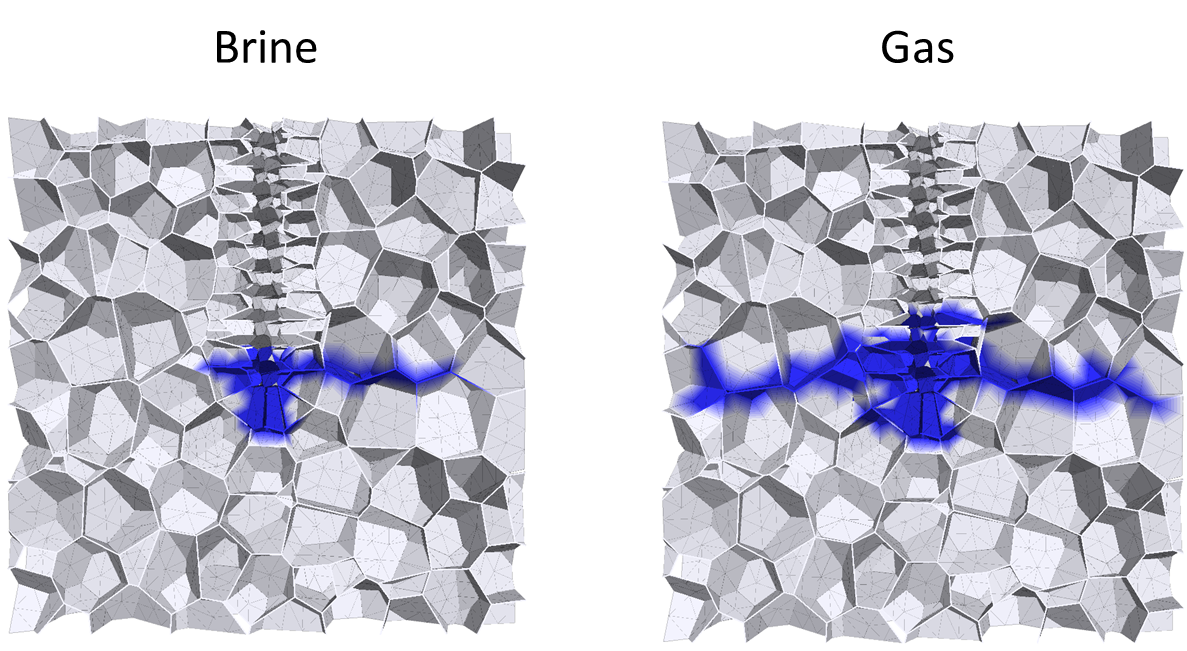
\includegraphics[width=1\textwidth]{figures/me4-3dec-vertcuts.png}
\caption{Final pressure distributions. The brine (left) gets stuck, the gas (right) reaches the boundaries and leaks out.}
\label{fig:ME4-3dec-vertcuts}
\end{figure}

Figure \ref{fig:ME4-3dec-comp} shows that there is a stark difference. The high bulk modulus of the brine leads to a very fast drop in pressure, while the gas pressure stays almost constant for quite a while. It should be mentioned that the timesteps do not correspond to a physical timescale, because the rate of the fluid flow between adjacent fluid knots in the model was artificially increased, and not derived from the aperture between two grains. Still, the qualitative difference persists. The brine pressure drops so fast, that the liquid becomes stuck inside the cube (Fig. \ref{fig:ME4-3dec-vertcuts} left), while the gas pressure decreases only after a significant amount leaked from the sample (Fig. \ref{fig:ME4-3dec-vertcuts} right). In addition, it should be noted that the brine pressure does not fall below 9.3 MPa, although the minimal principal stress is only 8 MPa. This is because of two effects: First, in order for pressure driven percolation to take place, the fluid pressure has to overcome the normal stress on the grain boundaries, which is a composition of all three external stresses due to the tilted orientations. Second, the fluid has to overcome the tensile strength, set to 1 MPa, of the joints, too. 

\subsubsection*{Lattice-Element-Method (LEM)}

In order to simulate the compressibility effect with lattice model, the similar setup as shown in Fig. \ref{fig:ME4-dem-setup} is considered. The initial reservoir pressure is set to be 12 $MPa$, which is higher than minimum principal stress of 8 $MPa$. The bulk modulus of brine is assumed to be 2 $GPa$ and the volume of reservoir to be 13 $L$. The total number of mechanical and conduct lattice elements are approximately 6000 and 45000, respectively. The rate of pressure drop in the reservoirs storing the brine and gas (methane) is investigated. The hydro model explained in section \ref{Section:HMLattice} is implemented to grant the mass conservation in the domain. The boundary reservoir pressure is not constant and with the fluid/gas transport in the medium it gradually drops. Due to the high bulk modulus of brine it is expected that the pressure drop in the brine reservoir to be higher than gas reservoir. However, the gas is leaked in higher rate where the kinematic viscosity is higher. Fig. \ref{fig:Amir_ME4_Brine_Frack} and Fig. \ref{fig:Amir_ME4_Brine_Flow} depict the fracking path (red) and flow rate in the flow channels (blue) for a brine reservoir. For a gas reservoir, Fig. \ref{fig:Amir_ME4_Gas_Frack} and Fig. \ref{fig:Amir_ME4_Gas_Flow} show the fracking path (red) and flow rate in the flow channels (blue). The amount of flow transport in the domain and in a same time step for a gas is higher than brine. \hl{Figure ???} illustrates the time dependent pressure drop for gas and brine reservoirs. As expected, the rate of pressure drop in the brine reservoir is much higher than gas reservoir.

\begin{figure}[!ht]
\begin{subfigure}[c]{0.48\textwidth}
\centering
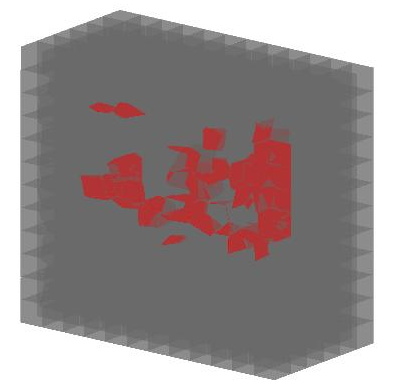
\includegraphics[width=5cm,height=5cm]{figures/Amir_ME4_Brine_Frack.png}
\subcaption{}
\label{fig:Amir_ME4_Brine_Frack}
\end{subfigure}
\hfill
\begin{subfigure}[c]{0.48\textwidth}
\centering
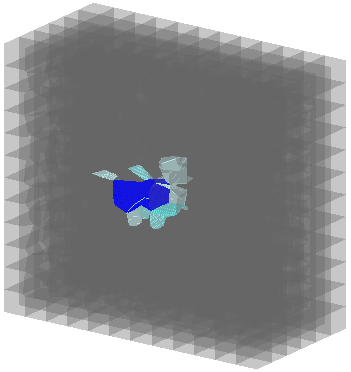
\includegraphics[width=5cm,height=5cm]{figures/Amir_ME4_Brine_Flow.png}
\subcaption{}
\label{fig:Amir_ME4_Brine_Flow}
\end{subfigure}
\caption{The (a) fracking path and (b) flow path for a brine reservoir}
\end{figure}

\begin{figure}[!ht]
\begin{subfigure}[c]{0.48\textwidth}
\centering
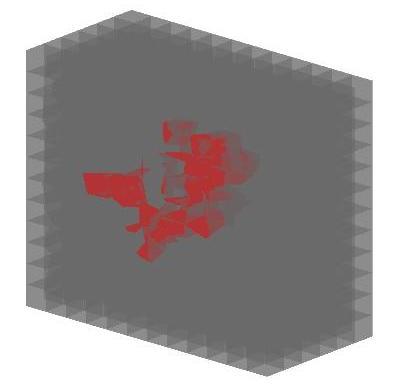
\includegraphics[width=5cm,height=5cm]{figures/Amir_ME4_Gas_Frack.png}
\subcaption{}
\label{fig:Amir_ME4_Gas_Frack}
\end{subfigure}
\hfill
\begin{subfigure}[c]{0.48\textwidth}
\centering
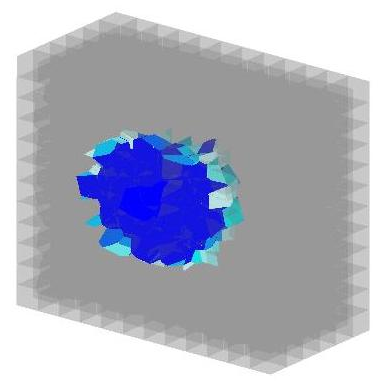
\includegraphics[width=5cm,height=5cm]{figures/Amir_ME4_Gas_Flow.png}
\subcaption{}
\label{fig:Amir_ME4_Gas_Flow}
\end{subfigure}
\caption{The (a) fracking path and (b) flow path for a gas reservoir}
\end{figure}

\subsubsection*{Finite-Element-Method: Variational Phase-Field}

The simulation set-up will be identical to Fig.~\ref{fig:VPF_init} except that the injection fluid will be compressible fluid (ideal gas). 


\subsection{Results and discussion}
%------------------------------------------------------------------------------
\todo[inline]{[IfG] Please add discussion}